\chapter{Probability Distributions}
\label{ch:probability-distributions}

\minitoc


This appendix gives the definitions and some properties of the probability distributions used for inference in this thesis. For each distribution, we list some key statistics such as the expectation, the variance (or covariance), and the entropy $\mathrm{H}(x)$.


\section{Uniform Distribution}
\label{sec:uniform-distribution}

The uniform distribution is often used as a non-informative prior, and assigns equal mass to all possible values in the distribution. When the variable is discrete, the probability is trivially set by dividing the total mass by the number of possible discrete values $N$,
\begin{equation}
	p(n) = \frac{1}{N},
\end{equation}
but when the variable is continuous, it can be more difficult to specify a density. Fortunately, when the range of possible values is limited to some interval, the density is given as
\begin{equation}
	\mathcal{U}(x|a, b)
	\equiv \frac{1}{b-a}\mathds{1}_{(a,\, b)}(x)
\end{equation}
which assigns equal mass within the interval and zero mass elsewhere. When a uniform distribution is required over all real values $x \in \mathbb{R}$, the distribution is \emph{improper} since it is impossible to normalise the density.

The mean and variance of the continuous uniform distribution are respectively:
\begin{equation}
\label{eq:uniform-moments}
	\mathbb{E}(x) = \frac{a+b}{2}
	\quad \text{and} \quad
	\mathrm{Var}(x) = \frac{(b-a)^2}{12}.
\end{equation}
An interesting property is that if $x$ has distribution $\mathcal{U}(x|0, 1)$, then $y \equiv a + (b-a)x$ will have distribution $\mathcal{U}(y|a, b)$.


\section{Gamma Distribution}

The Gamma is a probability distribution over a positive random variable $x > 0$ governed by a shape parameter $a$ and a rate parameter $b$ that are subject to the constraints $a > 0$ and $b > 0$ to ensure that the distribution can be normalised.
\begin{align}
	\mathcal{G}(x|a, b)
	&= \frac{b^a}{\Gamma(a)}x^{a-1}\exp\big\{-bx\big\}\mathds{1}_{(0,\,\infty)}(x)
	\label{eq:gamma-density} \\
	\mathbb{E}(x) &= \frac{a}{b}
	\\
	\mathrm{Var}(x) &= \frac{a}{b^2}
	\\
	\mathrm{mode}(x) &= \frac{a-1}{b}
	\qquad \text{for } a \geq 1,
\end{align}
where $\Gamma(a) = \int_{0}^{\infty} x^{a-1}\exp\big\{-x\big\}\,\mathrm{d}x$ is the gamma function.

The Gamma distribution is typically used as a prior for scale parameters (see e.g. \citep{berger85}). An example of scale parameter would be the standard deviation $\sigma$ of a univariate Gaussian distribution, after we have taken account of the location parameter $\mu$. The uninformative prior is obtained as the special case $a = b = 0$, in which $p(x) = \mathcal{G}(x|a, b)$ takes the form $p(x) \propto 1/x$. Using the transformation rule \eqref{eq:pdf-chg-of-vars} for densities, we see that this leads to a uniform prior over the logarithmic scale, i.e.\ $p(\log x) = \text{const}$.


\section{Shifted Exponential Distribution}
\label{sec:shifted-exponential-distribution}

An important special case of the Gamma distribution is the exponential distribution, whose density is obtained by setting $a = 1$ in Eq. \eqref{eq:gamma-density}:
\begin{equation}
	\mathcal{E}(x|\lambda)
	= \lambda\exp\Big\{-\lambda x\Big\}\mathds{1}_{(0,\,\infty)}(x),
\end{equation}
with $\lambda = \beta$. The exponential distribution is used to describe the time between events in a Poisson point process, i.e.\ a process in which events occur continuously and independently at a constant average rate $\lambda$.

If we shift the origin of an exponentially distributed random variable, then we obtain the so-called shifted exponential distribution, whose density is given by
\begin{equation}
	\mathcal{E}(x|\lambda, \theta)
	= \lambda\exp\Big\{-\lambda(x - \theta)\Big\}\mathds{1}_{(\theta,\, \infty)}(x),
\end{equation}
where, as before, $\lambda > 0$ is the rate parameter, while $\theta \in \mathbb{R}$ is the location parameter. The shifted exponential distribution is widely used in the analysis of lifetime or response time data that arises in areas such as product performance evaluation and clinical trials \citep{bain78, lawless82}. Using integration by parts, it is straightforward to show that its mean and variance are respectively:
\begin{equation}
\label{eq:shifted-exponential-moments}
	\mathbb{E}(x) = \frac{1}{\lambda} + \theta,
	\qquad
	\mathrm{Var}(x) = \frac{1}{\lambda^2}.
\end{equation}
Note that the variance coincides with that of the non-shifted exponential distribution, which is not surprising given that the variance is invariant to translations.


\section{Gaussian Distribution}

The Gaussian is the most widely used distribution for continuous variables. It is also known as the \emph{normal} distribution. In the case of a single variable $x \in \mathbb{R}$, it is governed by two parameters, the mean $\mu \in \mathbb{R}$ and the variance $\sigma^2 > 0$.
\begin{align}
	\mathcal{N}(x|\mu,\, \sigma^2)
	&= \frac{1}{\sqrt{2\pi\sigma^2}}\exp\Big\{-\frac{1}{2\sigma^2}(x - \mu)^2\Big\}
	\\
	\mathbb{E}(x) &= \mu
	\\
	\mathrm{Var}(x) &= \sigma^2
	\\
	\mathrm{mode}(x) &= \mu
	\\
	\mathrm{H}(x)
	&= \frac{1}{2}\log\sigma^2 + \frac{1}{2}[1 + \log(2\pi)].
\end{align}
The inverse of the variance $\beta = 1/\sigma^2$ is called the precision, and the square root of the variance, $\sigma$, is called the standard deviation.

For an $n$-dimensional column vector $\mathbf{x}$, the Gaussian is governed by an $n$-dimensional (column) mean vector $\boldsymbol{\mu}$ and an $n\times n$ covariance matrix $\boldsymbol{\Sigma}$ that must be symmetric and positive-definite.
\begin{align}
	\mathcal{N}(\mathbf{x}|\boldsymbol{\mu},\, \boldsymbol{\Sigma})
	&= (2\pi)^{-n/2}|\boldsymbol{\Sigma}|^{-1/2}\exp\Big\{-\frac{1}{2}(\mathbf{x} - \boldsymbol{\mu})^\text{T}\boldsymbol{\Sigma}^{-1}(\mathbf{x} - \boldsymbol{\mu})\Big\}
	\label{eq:gaussian-pdf-def} \\
	\mathbb{E}(\mathbf{x}) &= \boldsymbol{\mu}
	\\
	\mathrm{Cov}(\mathbf{x}) &= \boldsymbol{\Sigma}
	\\
	\mathrm{mode}(\mathbf{x}) &= \boldsymbol{\mu}
	\\
	\mathrm{H}(\mathbf{x})
	&= \frac{1}{2} \log|\boldsymbol{\Sigma}| + \frac{n}{2}[1 + \log(2\pi)].
	\label{eq:multivariate-gaussian-entropy}
\end{align}
The inverse of the covariance matrix $\boldsymbol{\Lambda} = \boldsymbol{\Sigma}^{-1}$ is the precision matrix, which is also symmetric and positive definite. Averages of random variables tend to a Gaussian, by the central limit theorem, and the sum of two Gaussian variables is again Gaussian. The Gaussian is the distribution that maximises the entropy for a given variance (or covariance).

Any linear transformation of a Gaussian random variable is again a Gaussian. The marginal distribution of a multivariate Gaussian with respect to a subset of the variables is itself Gaussian, and similarly the conditional distribution is also Gaussian. See below for details.

\subsection{Properties}
\label{sec:gaussian-identities}

The following properties \citep{rasmussen06, barber} are almost indispensable when dealing with Gaussian distributions.

\subsubsection{Completing the square}

A useful technique in manipulating Gaussians is the so-called technique of `completing the square'. For example, the expression
\begin{equation}
	\exp\Big\{-\frac{1}{2}\mathbf{x}^\text{T}\mathbf{A}\mathbf{x} + \mathbf{b}^\text{T}\mathbf{x}\Big\}
\end{equation}
can be transformed as follows. First, we complete the square with respect to $\mathbf{x}$ in the exponent:
\begin{equation}
	\frac{1}{2}\mathbf{x}^\text{T}\mathbf{A}\mathbf{x} - \mathbf{b}^\text{T}\mathbf{x}
	= \frac{1}{2}(\mathbf{x} - \mathbf{A}^{-1}\mathbf{b})^\text{T}\mathbf{A}(\mathbf{x} - \mathbf{A}^{-1}\mathbf{b}) - \frac{1}{2}\mathbf{b}^\text{T}\mathbf{A}^{-1}\mathbf{b}.
\end{equation}
Hence,
\begin{equation}
	\exp\Big\{-\frac{1}{2}\mathbf{x}^\text{T}\mathbf{A}\mathbf{x} + \mathbf{b}^\text{T}\mathbf{x}\Big\}
	= \mathcal{N}(\mathbf{x}|\mathbf{A}^{-1}\mathbf{b},\, \mathbf{A}^{-1})\sqrt{|2\pi\mathbf{A}^{-1}|}\exp\Big\{\frac{1}{2}\mathbf{b}^\text{T}\mathbf{A}^{-1}\mathbf{b}\Big\}.
\end{equation}
From this, one can derive
\begin{equation}
	\int \exp\Big\{-\frac{1}{2}\mathbf{x}^\text{T}\mathbf{A}\mathbf{x} + \mathbf{b}^\text{T}\mathbf{x}\Big\}\,\mathrm{d}\mathbf{x}
	= \sqrt{|2\pi\mathbf{A}^{-1}|}\exp\Big\{\frac{1}{2}\mathbf{b}^\text{T}\mathbf{A}^{-1}\mathbf{b}\Big\}.
\end{equation}

\subsubsection{Product of two Gaussians}

The product of two Gaussians is another Gaussian, with a multiplicative factor:
\begin{equation}
\label{eq:product-of-2-gaussians}
	\mathcal{N}(\mathbf{x}|\boldsymbol{\mu}_1,\, \boldsymbol{\Sigma}_1)\,\mathcal{N}(\mathbf{x}|\boldsymbol{\mu}_2,\, \boldsymbol{\Sigma}_2)
	= \mathcal{N}(\mathbf{x}|\boldsymbol{\mu},\, \boldsymbol{\Sigma})\frac{\exp\big\{-\frac{1}{2}(\boldsymbol{\mu}_1 - \boldsymbol{\mu}_2)^\text{T}\mathbf{S}^{-1}(\boldsymbol{\mu}_1 - \boldsymbol{\mu}_2)\big\}}{\sqrt{|2\pi\mathbf{S}|}},
\end{equation}
where $\mathbf{S} \equiv \boldsymbol{\Sigma}_1 + \boldsymbol{\Sigma}_2$ and the mean and covariance are given by
\begin{equation}
	\boldsymbol{\mu}
	= \boldsymbol{\Sigma}(\boldsymbol{\Sigma}_1^{-1}\boldsymbol{\mu}_1 + \boldsymbol{\Sigma}_2^{-1}\boldsymbol{\mu}_2)
	\qquad \text{and} \qquad
	\boldsymbol{\Sigma}
	= (\boldsymbol{\Sigma}_1^{-1} + \boldsymbol{\Sigma}_2^{-1})^{-1}.
\end{equation}
Note that the resulting Gaussian has a precision (inverse covariance) equal to the sum of the precisions, and a mean equal to the convex sum of the means, weighted by the precisions.

To prove Eq. \eqref{eq:product-of-2-gaussians}, simply write out the (lengthy) expressions by using the definition \eqref{eq:gaussian-pdf-def} of the Gaussian PDF, and expanding the terms inside the exponential to verify equality (hint: it may be helpful to expand $\boldsymbol{\Sigma}$ using the matrix inversion lemma in Eq. \eqref{eq:woodbury-identity}) 

\subsubsection{Affine transformations}

Any affine transformation of a Gaussian random vector is itself Gaussian. More precisely, if $\mathbf{y} \equiv \mathbf{A}\mathbf{x} + \mathbf{b}$ and $\mathbf{x} \sim \mathcal{N}(\mathbf{x}|\boldsymbol{\mu},\, \boldsymbol{\Sigma})$, where $\mathbf{x}$ is an $n$-dimensional column vector, $\mathbf{A}$ is a constant $m\times n$ matrix and $\mathbf{b}$ is an $m\times 1$ vector of constants, then $\mathbf{y}$ has multivariate Gaussian distribution with mean $\mathbf{A}\boldsymbol{\mu} + \mathbf{b}$ and covariance $\mathbf{A}\boldsymbol{\Sigma}\mathbf{A}^\text{T}$. In other words,
\begin{equation}
	\mathbf{x} \sim \mathcal{N}(\mathbf{x}|\boldsymbol{\mu},\, \boldsymbol{\Sigma})
	\quad \implies \quad
	\mathbf{y} \equiv \mathbf{A}\mathbf{x} + \mathbf{b}
	\sim \mathcal{N}(\mathbf{y}|\mathbf{A}\boldsymbol{\mu} + \mathbf{b},\, \mathbf{A}\boldsymbol{\Sigma}\mathbf{A}^\text{T}).
\end{equation}

\subsubsection{Partitioned Gaussians}

Perhaps the most important property of a multivariate Gaussian distribution is that its marginals and conditionals are both themselves Gaussian. That is, if we have a joint Gaussian distribution $\mathcal{N}(\mathbf{x}|\boldsymbol{\mu},\, \boldsymbol{\Sigma})$ with $\boldsymbol{\Lambda} \equiv \boldsymbol{\Sigma}^{-1}$ and we define the following partitions
\begin{align}
	& \mathbf{x} =
	\begin{pmatrix}
		\mathbf{x}_a \\
		\mathbf{x}_b
	\end{pmatrix},
	\qquad
	\boldsymbol{\mu} =
	\begin{pmatrix}
		\boldsymbol{\mu}_a \\
		\boldsymbol{\mu}_b
	\end{pmatrix}
	\\
	& \boldsymbol{\Sigma} =
	\begin{bmatrix}
		\boldsymbol{\Sigma}_{aa} & \boldsymbol{\Sigma}_{ab} \\
		\boldsymbol{\Sigma}_{ba} & \boldsymbol{\Sigma}_{bb}
	\end{bmatrix},
	\qquad
	\boldsymbol{\Lambda} =
	\begin{bmatrix}
		\boldsymbol{\Lambda}_{aa} & \boldsymbol{\Lambda}_{ab} \\
		\boldsymbol{\Lambda}_{ba} & \boldsymbol{\Lambda}_{bb}
	\end{bmatrix}	
\end{align}
then the conditional distribution $p(\mathbf{x}_a|\mathbf{x}_b)$ is given by
\begin{equation}
	p(\mathbf{x}_a|\mathbf{x}_b)
	= \mathcal{N}(\mathbf{x}_a|\boldsymbol{\mu}_{a|b},\, \boldsymbol{\Lambda}_{aa}^{-1}),
	\qquad
	\boldsymbol{\mu}_{a|b}
	= \boldsymbol{\mu}_{a} - \boldsymbol{\Lambda}_{aa}^{-1}\boldsymbol{\Lambda}_{ab}(\mathbf{x}_b - \boldsymbol{\mu}_{b})
\end{equation}
and the marginal $p(\mathbf{x}_a)$ is given by
\begin{equation}
	p(\mathbf{x}_a)
	= \mathcal{N}(\mathbf{x}_a|\boldsymbol{\mu}_{a},\, \boldsymbol{\Sigma}_{aa}).
\end{equation}

\subsubsection{Marginal and conditional Gaussians}

We now turn to another important property of the Gaussian distribution, illustrated in Figure~\ref{fig:mosb}.
\begin{figure}
\centering
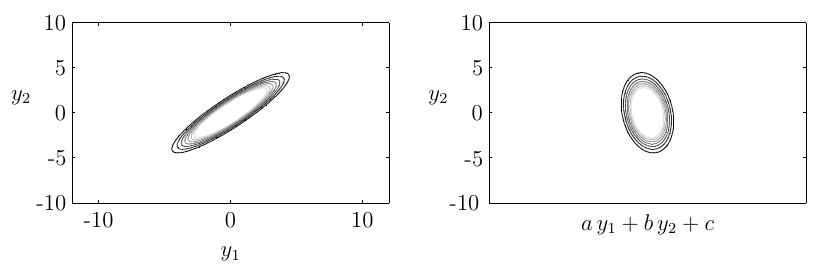
\includegraphics[scale=0.7]{mosb}
\caption{Any variables over which we have a multivariate Gaussian are jointly Gaussian with any linear transformation of those variables. Source: \citep{mosb}.}
\label{fig:mosb}
\end{figure}
Given a marginal Gaussian distribution for $\mathbf{x}$ and a conditional Gaussian distribution for $\mathbf{y}$ given $\mathbf{x}$ in the form
\begin{align}
	p(\mathbf{x}) &= \mathcal{N}(\mathbf{x}|\boldsymbol{\mu},\, \boldsymbol{\Lambda}^{-1})
	\\
	p(\mathbf{y}|\mathbf{x}) &= \mathcal{N}(\mathbf{y}|\mathbf{A}\mathbf{x} + \mathbf{b},\, \mathbf{L}^{-1})
\end{align}
the marginal distribution of $\mathbf{y}$ and the conditional distribution for $\mathbf{x}$ given $\mathbf{y}$ are given by
\begin{align}
	p(\mathbf{y}) &= \mathcal{N}(\mathbf{y}|\mathbf{A}\boldsymbol{\mu} + \mathbf{b},\, \mathbf{L}^{-1} + \mathbf{A}\boldsymbol{\Lambda}^{-1}\mathbf{A}^\text{T})
	\\
	p(\mathbf{x}|\mathbf{y}) &= \mathcal{N}(\mathbf{x}|\boldsymbol{\Sigma}\{\mathbf{A}^\text{T}\mathbf{L}(\mathbf{y} - \mathbf{b}) + \boldsymbol{\Lambda}\boldsymbol{\mu}\},\, \boldsymbol{\Sigma})
\end{align} 
where
\begin{equation}
	\boldsymbol{\Sigma} = (\boldsymbol{\Lambda} + \mathbf{A}^\text{T}\mathbf{L}\mathbf{A})^{-1}.
\end{equation}

\subsubsection{Gaussian average of a quadratic function}

Last but not least, the following result is also useful:
\begin{equation}
\label{eq:gaussian-avg-of-quadratic-fct}
	\langle\mathbf{x}^\text{T}\mathbf{A}\mathbf{x}\rangle_{\mathcal{N}(\mathbf{x}|\boldsymbol{\mu},\, \boldsymbol{\Sigma})}
	= \boldsymbol{\mu}^\text{T}\mathbf{A}\boldsymbol{\mu}
	+ \mathrm{Tr}(\mathbf{A}\boldsymbol{\Sigma}).
\end{equation}

\section{Generalised Gaussian Distribution}
\label{sec:generalised-gaussian-distribution}

The generalised inverse Gaussian distribution (GIG) is a three-parameter family of continuous probability distributions with probability density function
\begin{equation}
	\mathcal{GIG}(x|\delta, \chi, \psi)
	= \frac{(\psi/\chi)^{\delta/2}}{2K_{\delta}(\sqrt{\psi\chi})}x^{\delta-1}\exp\Big\{-\frac{1}{2}\left(\psi x + \frac{\chi}{x}\right)\Big\}\mathds{1}_{(0,\, \infty)}(x),
\end{equation}
where $K_{\delta}(\cdot)$ denotes the modified Bessel function of the second kind with index $\delta \in \mathbb{R}$, and $\chi, \psi > 0$. It is used extensively in geostatistics, statistical linguistics, finance, etc. Its statistical properties, and in particular the following lemma, can be found in \citep{jorgensen82}.
\begin{lemma}
\label{lem:jorgensen}
Let $x$ be distributed according to $\mathcal{GIG}(x|\delta, \chi, \psi)$, with $\psi > 0$ and $\chi > 0$. Then
\begin{equation}
	\mathbb{E}(x^p)
	= \left(\frac{\chi}{\psi}\right)^{p/2}\frac{K_{\delta+p}(\sqrt{\psi\chi})}{K_{\delta}(\sqrt{\psi\chi})}.
\end{equation}
\end{lemma}
An immediate consequence of this lemma that turns out to be useful for our purposes is given below. 
\begin{corollary}
\label{cor:jorgensen}
If $x$ is distributed according to $\mathcal{GIG}(x|1/2, \chi, \psi)$, where $\psi > 0$ and $\chi > 0$, then
\begin{align}
	\mathbb{E}(x)
	= \frac{1 + \sqrt{\psi\chi}}{\psi},
	\qquad
	\mathbb{E}(x^{-1})
	= \sqrt{\frac{\psi}{\chi}}.
\end{align}
\end{corollary}
It is straightforward to prove this corollary, by combining Lemma~\ref{lem:jorgensen} with the following one from \citep{abramowitz}.
\begin{lemma}
\label{lem:abramowitz}
The modified Bessel function of the second kind, $K_{\delta}(\cdot)$, satisfies the following properties:
\begin{enumerate}
	\item $K_{\delta}(x) = K_{-\delta}(x)$;
	\item $K_{\delta+1}(x) = 2\frac{\delta}{x}K_{\delta}(x) + K_{\delta-1}(x)$;
	\item $K_{1/2}(x) = K_{-1/2}(x) = \sqrt{\frac{\pi}{2x}}\exp\{-x\}$.
\end{enumerate}
\end{lemma}

\subsection{Entropy}

Using Lemmata~\ref{lem:jorgensen} and~\ref{lem:abramowitz}, the entropy of the generalised inverse Gaussian distribution is given as
\begin{align}
	\mathrm{H}(x)
	&= \frac{\delta}{2}\log\frac{\chi}{\psi} + \log\big[2K_{\delta}\big(\sqrt{\psi\chi}\big)\big] - (\delta-1)\langle\,\log x\,\rangle
	\nonumber \\
	& \quad + \frac{\sqrt{\psi\chi}}{2K_{\delta}(\sqrt{\psi\chi})}\big[K_{\delta+1}\big(\sqrt{\psi\chi}\big) + K_{\delta-1}\big(\sqrt{\psi\chi}\big)\big]
	\\	
	&= \frac{\delta}{2}\log\frac{\chi}{\psi} + \log\big[2K_{\delta}\big(\sqrt{\psi\chi}\big)\big] - (\delta-1)\frac{\frac{\mathrm{d}}{\mathrm{d}\nu}K_{\nu}(\sqrt{\psi\chi})\big|_{\nu=\delta}}{K_{\delta}(\sqrt{\psi\chi})}
	\nonumber \\
	& \quad + \frac{\sqrt{\psi\chi}}{2K_{\delta}(\sqrt{\psi\chi})}\big[K_{\delta+1}\big(\sqrt{\psi\chi}\big) + K_{\delta-1}\big(\sqrt{\psi\chi}\big)\big],
	\nonumber
\end{align}
where $\frac{\mathrm{d}}{\mathrm{d}\nu}K_{\nu}(\sqrt{\psi\chi})\big|_{\nu=\delta}$ is the derivate of the modified Bessel function of the second kind with respect to its order $\nu$, evaluated at $\nu=\delta$. In particular, when $\delta = 1/2$, this boils down to
\begin{equation}
\label{eq:gig-entropy}
	\mathrm{H}(x)
	= \frac{1}{2}\left(1 - \log\frac{\psi}{2\pi}\right) - (\delta-1)\langle\,\log x\,\rangle,
\end{equation}
which is easily proved by making use of Lemma~\ref{lem:abramowitz}.

\subsection{Special cases}

It is well know that the special cases of the GIG distribution include the Gamma distribution $\mathcal{G}(x|\delta, \psi/2)$ when $\chi = 0$ and $\delta > 0$, the inverse Gamma distribution $\mathcal{IG}(x|-\delta, \chi/2)$ when $\psi = 0$ and $\delta < 0$, the inverse Gaussian distribution when $\delta = -1/2$, and the hyperbolic distribution when $\delta = 0$. We refer the reader to \citep{jorgensen82} for details.

Note in particular that the PDF of the inverse Gaussian $\mathcal{GIG}(x|1/2, \chi, \psi)$ is
\begin{equation}
\label{eq:gig-pdf-for-delta-1/2}
	p(x)
	= \sqrt{\frac{\psi}{2\pi}}\exp\Big\{\sqrt{\psi\chi}\Big\}x^{-1/2}\exp\Big\{-\frac{1}{2}\left(\psi x + \frac{\chi}{x}\right)\Big\}\mathds{1}_{(0,\, \infty)}(x).
\end{equation}